\chapter{环境}

\section{为什么要自己排版?}
\label{sec:whyTypesetting}

如果是纯文学著作,完全可以交给出版社去排版。
但是对于编程技术书籍,文字之间还穿插代码和图表,
那么出版社的专业排版人员很难排出符合程序员审美观的版面,
甚至有可能造成技术错误。


\begindot
\item 代码的排版,注意分页和折行。特别是Python这种缩进敏感的语言,
一般要避免在一个函数内分页,这会造成阅读困难。可以在函数定义之间分页。

\item 写作与排版一体化,作者可以适当改写内容,让版面更美观。
例如,假如一个函数最后一行那个花括号被挤到了下一页第一行,这就很难看。
这时可以考虑临时改变代码的缩进(从BSD风格改为K\&R风格),从而节省一两行空间,
让花括号落在本页。另外也可以稍微改变说法,避免段尾孤字成行。

\item 文责自负,防止误改。例如我为某本书写的序言,其中提到旧的 boost \fn{RegEx}
\kw{class} 和新的 \fn{regex} \kw{class} 在线程安全性方面的不同。
这本书第二版再用这篇序言的时候被编辑“统一大小写”改为 \fn{RegEx},
整段话也就变得莫名其妙了。
类似的还有 $2^{32}-1$ 这种式子很容易被误改为 $232-1$,让人看了一头雾水。
\myenddot


\section{为什么要用\LaTeX排版?}
\begindot
\item \LaTeX 不会自作聪明地自动更正,例如句首字母大写
(关键字 \kw{double} 变为 \kw{Double}),
单词头两个字母大写(\fn{IUnknown} 变为 \fn{Iunknown}),
括号匹配(“[begin, end)”变为“[begin, end]”)等等。
Word 可以关闭自动更正,但是一旦整个流程(作者、编辑、校对、出片)中有一个人的设置不同,
稿子就有可能被误改。

\item \LaTeX 的源文件是文本格式,可以方便地做版本管理(\fn{diff}/\fn{merge}),
并且很容易利用和编写各种小工具来处理它。
相反Word的 \fn{.doc}/\fn{.docx} 文件处理起来就麻烦多了,如果不是不可能的话。
想想一句 \fn{grep | sort | uniq -c | sort -n} 要写多少代码。

\newpage
\item \LaTeX 可以处理英文断字(Hyphenation),避免一行文字太稀疏。
例如\fn{Concurrent\-Hash\-Map} 这种在技术书籍中经常出现的长类名,
如果不断字就会造成难看的版面。这也是Word排版容易出现的问题。
另外\LaTeX的断行和断页采用动态规划算法,排出来的版面比Word的贪心算法更匀称,
见后文的例子。


\item \LaTeX 可以方便地做出交叉引用,引用其他章节图表的页码或编号。
\LaTeX 原稿可以分散到多个 \fn{.tex} 文件中,便于编辑。
如果 Word 也这么做(每章一个文件),那么交叉引用就麻烦得多。
但是如果把整本书做成一个Word文件,那编辑起来就困难多了,牵一发而动全身。
而且有一种如履薄冰的感觉,生怕哪天文件突然就损坏了。
\myenddot

以下展示动态规划与贪心算法的区别。这里版心宽度是20个汉字。\label{ex:dynamicProgramming}
第一行排满了20字,刚刚好。
第二行排了16字,后接一个长单词,其宽度超过5个汉字,
因此本行排不下了。Word和\LaTeX都会把长单词移到第三行,
但是区别在于Word不会返回去调整第一行已经排好的那20个字%
(贪心算法只管当前行,排满为止,排不下就另起一行),
因此第二行比第一行显得稀疏,版面不匀称。
而 \LaTeX 则会把整个段落通盘考虑,它会从第一行挪两个字到第二行,
让前两行的字距相当,版面更匀称。

\vspace{1ex}
\centerline{
\includegraphics[page=2]{linebreak-crop.pdf}}

\subsection{动手之前}
作者有能力并且有意愿完整书籍的排版,向出版社提供印刷质量的PDF文稿。
出版社愿意改变通常的工作流程,采用作者提供的PDF文件来校对并印刷。
要事先沟通好。
\LaTeX 不是一个傻瓜化的工具,它需要投入相当的精力去学习,才能排出满意的效果。

%\section{硬件设备}
%我自己使用两台24吋显示器,并排

\section{软件工具}

\subsection{操作系统}

操作系统应满足三个条件:
有好用的中文输入法,有好用的PDF阅读器,
能方便地用命令行处理文本文件(\fn{grep}、\fn{sort}、\fn{awk} 等)。
目前看来符合这个条件的操作系统是Mac~OS X,
但是我不可能为了写一本书去买一台新的笔记本电脑。
因此我用的是一种混合办法,笔记本上安装Windows,
再在虚拟机中安装Debian Linux,
然后在Debian 中安装 TeX Live。
最后用Samba共享文件夹,这样就可以在Windows下方便地编辑Linux上的文件。
而在Linux上用 Git 管理 \fn{.tex} 源文件和图片,并且编译出PDF。

\subsection{\TeX 发行版}
Linux用TeX Live,Windows用CTeX套装,Mac~OS X 用 Mac TeX。
中文处理采用xelatex + xeCJK + ctex 方案
\footnote{\myurl{http://blog.jjgod.org/2009/11/21/chinese-in-tex-live-2009/}},
不要采用过时的 CJK 或 CCT 方案。

注意,\TeX本身是非常稳定的,但是中文处理则在不断改进。
例如TeX Live 2010和TeX Live 2012在处理中英文混排方面就有区别,
造成“动版”,严重时会影响既有分页。

\vspace{1ex}
\centerline{\fbox{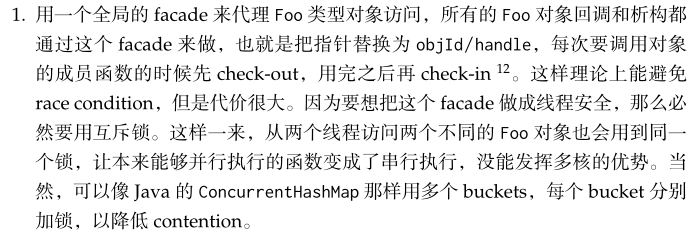
\includegraphics[width=360pt]{texlive2010.png}}}

\vspace{1ex}
\centerline{\fbox{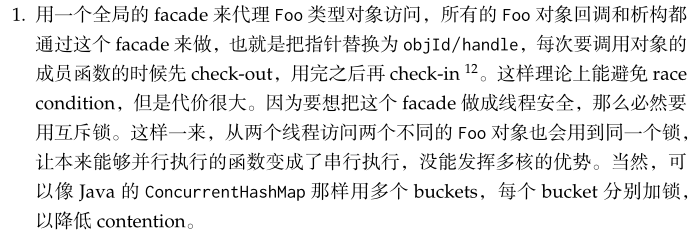
\includegraphics[width=360pt]{texlive2012.png}}}

\vspace{1ex}
因此我建议不要在排版期间升级 \LaTeX 的大版本,
这也是我在虚拟机上安装 TeX Live 的原因之一。
这样可以轻松地备份整个系统,
将来重印需要修订书中某几页的时候可以使用当年的虚拟机映像,版本一致,不必担心其他页面发生“动版”。

\subsection{PDF阅读器}
推荐SumatraPDF,它不锁PDF文件,可以随时覆盖,并且自动刷新。

\subsection{离线备份}
写书是一项耗时的任务,数据备份是必不可少的,
防止误操作和硬件损坏带来的不可弥补的损失。
除了 \S \ref{sec:versionControl} 讲的源文件版本管理之外,
各种图片、表格,以及生成PDF也要及时备份,
最好是离线(offline)备份。
可用以下这些网盘:

\begindot
\item Amazon Cloud Drive
\item Dropbox
\item Google Drive
\item Microsoft Sky Drive
\myenddot

这几个网盘都有Windows和Mac客户端,
这也是我使用Windows桌面的原因之一。

\section{版本管理}
\label{sec:versionControl}


我用Git管理 \fn{.tex} 文件和其他输入文件,
并且同步到 Github 的私人仓库,
就像这篇文章一样。

\subsection{理想的工作流程}
作者和编辑都使用版本管理软件,就像开发软件那样工作。
\LaTeX 就好比是编译器,
\fn{.tex} 文件是源程序,
\fn{.pdf} 文件是编译的结果。
作者和编辑都可以修改源程序,并且通过版本管理软件来merge结果。
考虑到作者和编辑不在同一个内网,因此一般要用公共的版本库,例如Github。
GitHub 的私有 repository 可保证数据安全。

\subsection{现实的工作流程}
编辑往往既不会\LaTeX也不会Git,那就之好采用原始方案,
作者提供PDF,编辑加以评注,或者打印出来再用红笔校对。

\section{\fn{.tex} 文件组织}
\fn{.tex} 文件一律使用 UTF-8编码,一来避免各种编码转换的问题(某些人名用字在GB2312中没有定义),
二来可以直接使用现有的Linux命令行工具来处理 \fn{.tex} 文件。
\fn{.tex} 文件一般可以按章或按节划分,每个文件不超过1000行,以利于编辑。
再用一个 \fn{.tex} 文件把它们 \mn{include} 到一起。
\fn{.tex} 和图片文件的文件名不要有下划线。
